\documentclass[a4paper,11pt,eval]{nsi} 
\usepackage{fontawesome5}

%\pagestyle{empty}


\newcounter{exoNum}
\setcounter{exoNum}{0}
%
\newcommand{\exo}[1]
{
	\addtocounter{exoNum}{1}
	{\titlefont\color{UGLiBlue}\Large Exercice\ \theexoNum\ \normalsize{#1}}\smallskip	
}



\begin{document}



\textcolor{UGLiBlue}{Vendredi 28/03/2025}\\
\classe{\terminale Comp}
\titre{Évaluation-bilan 5}
\maketitle
\begin{center}
	Calculatrice autorisée. Toutes les réponses doivent être justifiées.
\end{center}

%\vspace*{1cm}

\exo{}\bareme{8 pts}
\begin{enumerate}
    \item Soit $f$ la fonction définie sur $\fif{1}{20}$ par $f(x) = \dfrac{x+1-\ln(x)}{x}$.
    \begin{enumalph}
        \item Démontrer que, pour tout réel $x$ de $\fif{1}{20} : \quad f'(x) = \dfrac{-2+\ln(x)}{x^2}$.
        \item Résoudre dans $\fif{1}{20}$ l'inéquation $-2+\ln(x)> 0$.
        \item En déduire le tableau de variations de $f$ sur $\fif{1}{20}$.
    \end{enumalph}
    \carreauxseyes{16cm}{14.4cm}\\
    \carreauxseyes{16cm}{6.4cm}
    \item Une entreprise fabrique chaque jour entre 100 et 2000 pièces electroniques.\\
    On admet que lorsque $x$ centaines de pièces sont fabriquées, avec $1\leqslant x\leqslant 20$, le coût moyen de fabrication d'une pièces est de $f(x)$ euros, où $f$ est la fonction définie à la question précédente.
    \begin{enumalph}
        \item Déterminer, à l'unité près, le nombre de pièces à fabriquer pour que le coût moyen de fabrication d'une pièce soit minimal. Déterminer alors ce coût moyen, au centime d'euro près.
        %\item Déterminer le nombre minimal de pièces à fabriquer pour que le coût moyen de fabrication d'une pièce soit inférieur ou égal à 1,50 €.
        \item Est-il possible que le coût moyen d'une pièce soit de 50 centimes ? Justifier.
    \end{enumalph}
    \carreauxseyes{16cm}{14.4cm}
\end{enumerate}

\newpage
\exo{}\bareme{6 pts}\\
En mai 2020, une entreprise fait le choix de développer le télétravail afin de s'inscrire dans une démarche écoresponsable. Elle propose alors à ses \np{5000}~collaborateurs de choisir entre le télétravail et le travail au sein des locaux de l'entreprise.

Le nombre de collaborateurs en télétravail le $n$-ième mois après le mois de mai 2020 est modélisé par la suite $\left(a_n\right)$ définie sur $\N$ par : $$a_n = \np{- 2800} \times  0,85^n + \np{3000}$$
\begin{enumerate}

    \item \begin{enumalph}
        \item Calculer $a_0$ et $a_1$ puis interpréter ces résultats dans le contexte de l'exercice.
        \item Déterminer le sens de variation et la limite de la suite $(a_n)$.
    \end{enumalph}
    \item L'entreprise souhaite de changer de locaux lorsque la moitié de ses collaborateurs seront en télétravail. Elle veut prévoir la date à laquelle organiser ce déménagement.
    \begin{enumalph}
        \item Utiliser la fonction $\ln$ pour résoudre dans $\N$ l'inéquation $\np{- 2800} \times  0,85^n + \np{3000}>2500$.
        \item Interpréter le résultat dans le contexte de l'exercice.
    \end{enumalph}
\end{enumerate}
\carreauxseyes{16.8cm}{16.8cm}\\
\carreauxseyes{16.8cm}{9.6cm}

\vspace*{1cm}

\exo{}\bareme{6 pts}\\
Le niveau sonore $N$, en décibels (dB), d'un bruit, à une distance $D$, en m, de sa source, dépond de la puissance sonore $P$, en watts (W), de la source. Il est donnée par la relation :
$$N=120+4\ln\left(\dfrac{P}{13\times D^2}\right)$$
\begin{enumerate}
    \item On donne $N=76$ dB et $D=100$ m. Calculer la puissance sonore $P$, arrondir au centième.
    \item Sur le chantier d'une entreprise de travaux publics, une machine de découpe a une puissance sonore égale à $0,039$ W.
    \begin{enumalph}
        \item Montrer qu'à une distance $D$ de la machine, le niveau sonore $N$ dû à celle-ci vérifie la relation $N=120+4\ln(0,003)-4\ln\left(D^2\right)$.
        \item Montrer qu'une approximation de $N$ est $N\approx 96,76-8\ln(D)$.
    \end{enumalph}
    \item \textbf{Dans cette question, on utilisa l'approximation $N\approx 96,76-8\ln(D)$.}\\
    Un ouvrier doit porter des protection individuelles contre le bruit dès qu'un risque apparaît.
    \tabstyle[UGLiOrange]
    \begin{center}
        \begin{tabular}{|c|c|}
            \hline
            \ccell Impact sur l'audition & \ccell Niveaux sonores (en dB) \\\hline
            Aucun & $\fio{0}{85}$ \\\hline
            Risque faible & $\fio{85}{90}$ \\\hline
            Risque élévé & $\fio{90}{120}$ \\\hline
        \end{tabular}
    \end{center}
    \begin{enumalph}
        \item Justifier, à l'aide du tableau ci-dessus qu'un ouvrier de cette entreprise se situant à 3m de la machine doive porter des protections individuelles contre le bruit.
        \item Déterminer la distance à partir de laquelle un ouvrier sort de la zone de risque élevé. Arrondir au dm.
    \end{enumalph}
\end{enumerate}
\carreauxseyes{16.8cm}{25.6cm}

\newpage
\setcounter{exoNum}{0}

\titre{Corrigé - Éval-bilan 5}
\maketitle

\textcolor{UGLiBlue}{
    \exo{}
    \begin{enumerate}
        \item 
        \begin{enumalph}
            \item Soit $x\in\fif{1}{20}$.
            \begin{tabbing}
                $f(x) = \dfrac{u(x)}{v(x)}\quad$ avec$\quad$ \= $u(x) = x+1-\ln(x)\quad$ \= et $\quad v(x) = x$\\
                \>$u'(x) = 1-\dfrac{1}{x}$ \> et $\quad v'(x) = 1$\\
            \end{tabbing}
            \begin{tabbing}
                D'où $\quad f'(x)$\= $= \dfrac{u'(x)v(x)-u(x)v'(x)}{v(x)^2}$\\[.5em]
                \> $= \dfrac{\left(1-\dfrac{1}{x}\right)x - (x+1-\ln(x))}{x^2}$\\[.5em]
                \> $= \dfrac{x-1 - x - 1 + \ln(x)}{x^2}$\\[.5em]
                \> $= \dfrac{-2+\ln(x)}{x^2}$
            \end{tabbing}
            \item \begin{tabbing}
                Soit $x\in\fif{1}{20}, \quad -2+\ln(x)> 0\quad$ \= $\iff \quad \ln(x)>3$\\
                \> $\iff \quad x> e^2 \qquad$Or $e^2\approx 7,3891$\\
                \> $\iff \quad x\in\oif{e^2}{20}$
            \end{tabbing}
            \item Pour $x\in\fif{1}{20}, x^2>0$ donc $f'(x)$ est du signe de $-2+\ln(x)$.\\
            On en déduit le tableau de variations suivant :
            \begin{center}
                \begin{tikzpicture}
                    \tkzTabInit[color,lgt=3,espcl=3]
                    {$x$ / 1 , Signe de $f'(x)$ / 1, Variations de $f$ / 2}
                    {$1$, $e^2$, $20$}
                    \tkzTabLine{, -, z, +, }
                    \tkzTabVar{+/$2$ , -/$1-e^{-2}$ , +/$1.05-0.05\ln 20$}
                \end{tikzpicture}
            \end{center}
        \end{enumalph}
        \item \begin{enumalph}
            \item La fonction $f$ admet un minimum sur $\fif{1}{20}$ en $e^2\approx 7,39$ et $f(e^2) = 1-e^{-2}\approx 0,86$.\\
            Le coût moyen de fabrication d'une pièce est minimal pour 739 pièces produites et vaut environ 0,86 €.
            \item Le coût moyen d'une pièce ne peut pas être de 0,50 € car $0,50<1-e^{-2}\approx 0,86$.
        \end{enumalph}
    \end{enumerate}
    \exo{}
    \begin{enumerate}
        \item \begin{enumalph}
            \item $u_0 = -140\times 0,9^0+420 = -140\times 1+420 = -140+420 = 280$\\
            $u_1 = -140\times 0,9^1+420 = -140\times 0,9+420 = -126+420=294$.\\
            La commune loue 280 vélos en janvier 2025 et 294 vélos en février 2025.
            \item Soit $n\in\N$.\\
            $u_{n+1}-u_n = -140\times 0,9^{n+1}+420 - (-140\times 0,9^n+420)$\\
            $\phantom{u_{n+1}-u_n}= -140\times 0,9^n\times 0,9+420 + 140\times 0,9^n-420$\\
            $\phantom{u_{n+1}-u_n}= -140\times 0,9^n\times 0,9+140\times 0,9^n\times 1$\\
            $\phantom{u_{n+1}-u_n}= -140\times 0,9^n\times (0,9-1)$\\
            $\phantom{u_{n+1}-u_n}= -140\times 0,9^n\times (-0,1)$\\
            $\phantom{u_{n+1}-u_n}= 14\times 0,9^n$\\
            Donc $u_{n+1}-u_n>0$ et la suite $(u_n)$ est croissante.\\
            De plus, $\lim\limits_{n\to+\infty}u_n = -140\times 0,9^n+420 = 420$.
        \end{enumalph}
        \item \begin{enumalph}
            \item Soit $n\in\N$.
            \begin{tabbing}
                $-140\times 0,9^n+420>380 \quad$    \= $\iff\quad -140\times 0,9^n> -40 \qquad$ \= \\
                \>  $ \iff \quad 0,9^n<\dfrac{40}{140}$\\
                \> $ \iff \quad 0,9^n<\dfrac{2}{7}$.\\
                \> $ \iff \quad \ln(0,9^n)<\ln\left(\dfrac{2}{7}\right)$ \> car $\ln$ est croissante sur $\oio{0}{+\infty}$
                \\
                \> $ \iff \quad n\ln(0,9)<\ln\left(\dfrac{2}{7}\right)$\\
                \> $ \iff \quad n>\dfrac{\ln\left(\dfrac{2}{7}\right)}{\ln(0,9)}$ \> car $\ln(0,9)<0$\\
                \> $\iff\quad n\geqslant 12$.
            \end{tabbing}
            \item À partir du 12$^{\text{e}}$ mois soit janvier 2026, le nombre de vélos sera insuffisant.
        \end{enumalph}
    \end{enumerate}
    \exo{}
    \begin{enumerate}
        \item Pour $N=84$ dB et $D=10$ m, on a :
        \begin{tabbing}
            $84=120+4\ln\left(\dfrac{P}{13\times 10^2}\right)$ \= $\iff \quad -36 = 4\ln\left(\dfrac{P}{1300}\right)$\\
            \> $\iff \quad -9 = \ln\left(\dfrac{P}{1300}\right)$\\
            \> $\iff \quad e^{-9} = \dfrac{P}{1300}$\\
            \> $\iff \quad P = 1300e^{-9}$\\
            \>  $\iff \quad P\approx 0,16$ W.
        \end{tabbing} 
        \item \begin{enumalph}
            \item Pour $P=0,026$ W, on a :\\[.5em]
            $N=120+4\ln\left(\dfrac{0,026}{13\times D^2}\right)$\\
            $\phantom{N}=120+4\ln\left(\dfrac{0,002}{D^2}\right)$\\
            $\phantom{N}=120+4\ln(0,002)-4\ln(D^2)$
            \item $N= 120+4\ln(0,002)-4\ln(D^2)$\\
            $N= 120+4\ln(0,002)-4\times 2\ln(D)$\\
            $N\approx 95,14-8\ln(D)$.
        \end{enumalph}
\newpage
        \item \begin{enumalph}
            \item Pour $D=3$ m, on a :
            \begin{tabbing}
                $N$  \=$\approx 95,14-8\ln(3)$\\
                \>$\approx 95,14-8\times 1,099$\\
                \>$\approx 86,35$ dB.
            \end{tabbing}
            L'ouvrier doit porter des protections individuelles car $85<N<90$ dB.
            \item \begin{tabbing}
                $N<90\quad$ \= $\iff \quad 95,14-8\ln(D)<90$\\
                \> $\iff \quad -8\ln(D)<-5,14$\\
                \> $\iff \quad \ln(D)>\dfrac{5,14}{8}$\\
                \> $\iff \quad D>e^{\frac{5,14}{8}}$\\
                \> $\iff \quad D>e^{0,6425}$\\
                \> $\iff \quad D>1,9$
            \end{tabbing}
            L'ouvrier sort de la zone de risque élevé à partir de 1,9 m.
        \end{enumalph}
    \end{enumerate}
}
\end{document}